% ARCS: Autoregressive Representation for Circuit Synthesis
% Targeting ICCAD 2026
\documentclass[conference]{IEEEtran}

\usepackage{amsmath,amssymb}
\usepackage{graphicx}
\usepackage{booktabs}
\usepackage{hyperref}
\usepackage{xcolor}
\usepackage{algorithm}
\usepackage{algorithmic}
\usepackage{multirow}
\usepackage[normalem]{ulem}  % for \sout strikethrough
\usepackage{subcaption}
\usepackage{tikz}
\usepackage{pgfplots}
\pgfplotsset{compat=1.18}
\usetikzlibrary{arrows.meta,positioning,shapes.geometric,fit,calc,backgrounds,patterns}

\title{ARCS: Autoregressive Circuit Synthesis with\\
Topology-Aware Graph Attention and Spec Conditioning}

\author{
\IEEEauthorblockN{Tushar Pathak}
\IEEEauthorblockA{New York University\\
\texttt{tp2578@nyu.edu}}
}

\begin{document}
\maketitle

% ==========================================================================
\begin{abstract}
We present ARCS, an autoregressive transformer that generates complete
analog circuits---topology \emph{and} component values---in a single
forward pass conditioned on target specifications. ARCS uses a native
component-token vocabulary and a topology-aware Graph Transformer with
circuit-graph inductive bias. We identify a critical failure mode of
REINFORCE RL---cross-topology reward mismatch---and introduce
\emph{Group Relative Policy Optimization (GRPO)} with per-topology
advantage normalization, achieving 58.8\% simulation validity
(+14.4\,pp over REINFORCE) in only 500 RL steps.
\emph{Grammar-constrained decoding} guarantees 100\% structural
validity by construction via topology-aware token masking.
We additionally propose \emph{Constrained Circuit Flow Matching (CCFM)},
a non-autoregressive generator achieving 100\% structural validity
across 32 topologies. A hybrid pipeline combining learned generators
with SPICE-based ranking achieves 99.9\% simulation validity and
spec-aware reward 6.43/8.0 using only 8 SPICE evaluations---40$\times$
fewer than genetic algorithms. ARCS generates designs in $\sim$20\,ms
(generation only; SPICE verification adds $\sim$1\,s), over three orders
of magnitude faster than search-based alternatives.
\end{abstract}

% ==========================================================================
\section{Introduction}
\label{sec:intro}

Analog circuit design remains a manual, expertise-intensive process.
Engineers select a topology, choose component values, simulate, and
iterate---a cycle that can take days or weeks. Recent machine learning
approaches have begun to automate parts of this workflow, but each has
significant limitations.

\textbf{Topology-only generation.} AnalogGenie~\cite{analoggenie}
generates circuit topologies using an autoregressive transformer over
pin-level Eulerian sequences, achieving 93.2\% validity after PPO
fine-tuning. However, it produces no component values---a separate
genetic algorithm must size every generated circuit, adding minutes
of computation. It also lacks specification conditioning: circuits are
generated randomly, then filtered post-hoc.

\textbf{Text-based generation.} CircuitSynth~\cite{circuitsynth} and
AutoCircuit-RL~\cite{autocircuitrl} fine-tune large language models
(GPT-Neo, 2.7B parameters) on raw SPICE netlist text. These models
predict characters, not circuit components, leading to syntax errors in
generated netlists and no semantic understanding of component values.

\textbf{This work.} We propose ARCS (Figure~\ref{fig:overview}), which addresses all three gaps
simultaneously:
\begin{enumerate}
    \item \textbf{Native component-token vocabulary with topology-aware
    Graph Transformer}: Each token represents a circuit element paired
    with a discretized value, and a Graph Transformer injects
    circuit-graph structure via learned adjacency biases and RWPE,
    improving simulation validity by +6.2\,pp over the baseline.
    \item \textbf{Grammar-constrained decoding}: A state-machine-based
    token masking scheme guarantees 100\% structural validity \emph{by
    construction}, without RL training or post-hoc filtering.
    \item \textbf{Group Relative Policy Optimization (GRPO)}: A
    per-topology RL algorithm inspired by Shao~\emph{et~al.}~\cite{shao2024grpo},
    where advantages are z-scored within topology groups, resolving
    cross-topology reward mismatch and achieving 58.8\% simulation
    validity (+14.4\,pp over REINFORCE) with 10$\times$ fewer RL steps.
    \item \textbf{Constrained Circuit Flow Matching (CCFM)}: A
    non-autoregressive generator combining conditional flow matching
    with a circuit VAE and constraint-guided ODE sampling,
    achieving 100\% structural validity on 32 topologies.
    \item \textbf{Hybrid pipeline with inference-time scaling}:
    Multi-source ranking (VCG + CCFM + learned reward model) achieves
    99.9\% simulation validity and reward 6.43/8.0 with only 8 SPICE
    evaluations---40$\times$ fewer than genetic algorithm baselines.
\end{enumerate}

The key contribution of ARCS is not higher per-design quality than
search-based methods, but rather \emph{amortized inference}: a trained
model that produces reasonable first-shot designs in $\sim$20\,ms,
enabling rapid prototyping and design-space exploration at a cost
$>$10,000$\times$ lower than conventional search. We additionally show
that ARCS-generated designs can seed search methods (warm-start GA),
reducing simulation budgets by 49\% while retaining 96\% of the
optimality achieved by cold-start search.

\begin{figure*}[t]
\centering
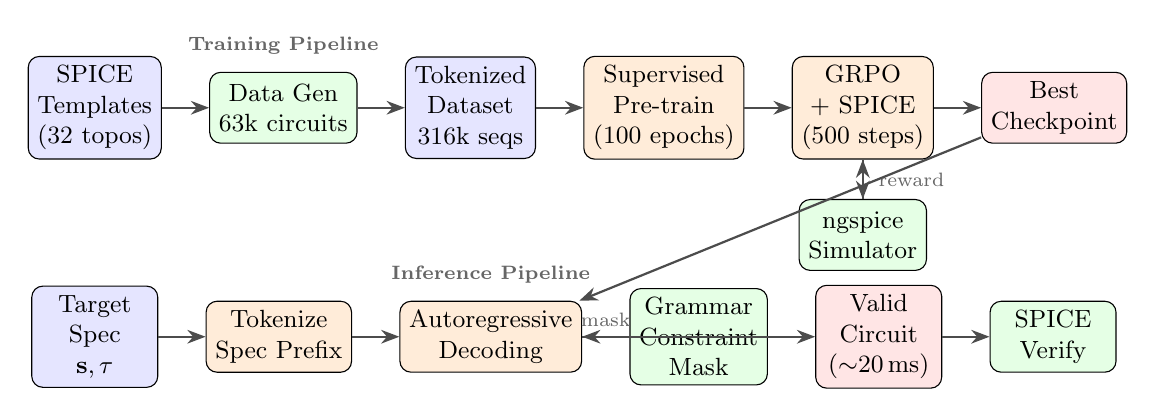
\begin{tikzpicture}[>=Stealth, node distance=0.6cm,
  block/.style={draw, rounded corners, minimum height=0.9cm,
    minimum width=1.6cm, align=center, font=\small},
  data/.style={block, fill=blue!10},
  model/.style={block, fill=orange!15},
  process/.style={block, fill=green!10},
  result/.style={block, fill=red!10},
  arr/.style={->, thick, color=black!70},
  lbl/.style={font=\scriptsize, color=black!60}
]
% Row 1: Training pipeline
\node[data] (templates) {SPICE\\Templates\\(32 topos)};
\node[process, right=of templates] (datagen) {Data Gen\\63k circuits};
\node[data, right=of datagen] (dataset) {Tokenized\\Dataset\\316k seqs};
\node[model, right=of dataset] (sl) {Supervised\\Pre-train\\(100 epochs)};
\node[model, right=of sl] (rl) {GRPO\\+ SPICE\\(500 steps)};
\node[result, right=of rl] (ckpt) {Best\\Checkpoint};

\draw[arr] (templates) -- (datagen);
\draw[arr] (datagen) -- (dataset);
\draw[arr] (dataset) -- (sl);
\draw[arr] (sl) -- (rl);
\draw[arr] (rl) -- (ckpt);

% Feedback loop from RL to SPICE
\node[process, below=0.5cm of rl] (spice) {ngspice\\Simulator};
\draw[arr] (rl) -- (spice);
\draw[arr] (spice) -- node[lbl,right,xshift=2pt]{reward} (rl);

% Row 2: Inference pipeline
\node[data, below=1.6cm of templates] (spec) {Target\\Spec\\$\mathbf{s},\tau$};
\node[model, right=of spec] (encode) {Tokenize\\Spec Prefix};
\node[model, right=of encode] (decode) {Autoregressive\\Decoding};
\node[process, right=of decode] (constrain) {Grammar\\Constraint\\Mask};
\node[result, right=of constrain] (circuit) {Valid\\Circuit\\($\sim$20\,ms)};
\node[process, right=of circuit] (verify) {SPICE\\Verify};

\draw[arr] (spec) -- (encode);
\draw[arr] (encode) -- (decode);
\draw[arr] (constrain) -- node[lbl,above]{mask} (decode);
\draw[arr] (decode) -- (circuit);
\draw[arr] (circuit) -- (verify);
\draw[arr] (ckpt) -- (decode);

% Labels
\node[lbl, above=0.1cm of datagen] {\textbf{Training Pipeline}};
\node[lbl, above=0.1cm of decode] {\textbf{Inference Pipeline}};
\end{tikzpicture}
\caption{ARCS system overview. \textbf{Top}: Training pipeline---SPICE
templates generate data, supervised pre-training learns the sequence
distribution, and GRPO with SPICE-in-the-loop per-topology advantages
refines value quality. \textbf{Bottom}: Inference pipeline---a target
specification is tokenized, the trained model autoregressively generates
component tokens with grammar-constrained masking, producing a valid
circuit in $\sim$20\,ms.}
\label{fig:overview}
\end{figure*}

% ==========================================================================
\section{Related Work}
\label{sec:related}

\subsection{Autoregressive Circuit Generation}

AnalogGenie~\cite{analoggenie} introduced Eulerian circuit representations
for autoregressive generation, training a GPT decoder (11.8M parameters)
on 3,502 circuits manually curated from IEEE publications.
After PPO fine-tuning, it achieves 93.2\% structural validity. Key
limitations: no component values in the vocabulary, no specification
conditioning, and reliance on a GA for post-hoc sizing.

CircuitSynth~\cite{circuitsynth} and AutoCircuit-RL~\cite{autocircuitrl}
fine-tune GPT-Neo (2.7B parameters) on SPICE netlist text, treating
circuit generation as a text completion task. While this includes
component values in the output, the model operates at the character
level with no circuit-specific inductive bias.

LaMAGIC~\cite{lamagic} generates analog IC topologies using language
models with graph-based representations. While it introduces
circuit-aware tokenization, it targets transistor-level IC design
rather than board-level circuits with discrete component values.
INSIGHT~\cite{insight} uses an autoregressive transformer as a
fast surrogate for SPICE simulation, achieving near-simulator
accuracy at orders-of-magnitude lower cost; however, it is a
\emph{predictor} of circuit performance, not a \emph{generator}
of new designs.

\subsection{Circuit Sizing and Optimization}

AutoCkt~\cite{autockt} uses deep reinforcement learning for analog
circuit sizing, treating component values as a continuous action space.
Wang~\emph{et~al.}~\cite{wang2020gcnrl} combine graph neural networks
with RL for transferable transistor sizing across circuit topologies.
Lyu~\emph{et~al.}~\cite{lyu2018weibo} apply Bayesian optimization
to analog sizing, achieving efficient exploration with Gaussian process
surrogate models.
CktGNN~\cite{cktgnn} uses graph neural networks for topology generation
but is limited to operational amplifiers.
Fan~\emph{et~al.}~\cite{fan2024graph} propose a graph-transformer
surrogate model for power converter topologies, achieving strong
prediction accuracy but focusing on evaluation rather than generation.
FALCON~\cite{falcon} combines GNN-based prediction with layout
co-optimization but is not generative for new topologies.

\subsection{Flow-Based Generative Models}

Conditional flow matching (CFM)~\cite{lipman2023flow} learns
continuous-time transport maps between a prior and data distribution
via optimal-transport velocity fields, avoiding the mode-collapse
issues of diffusion models and the KL-constrained latent space of
VAEs. CFM has been applied to molecular generation~\cite{song2024equivariant}
and protein design but, to our knowledge, not to circuit synthesis.
For discrete graph generation, DiGress~\cite{vignac2023digress} applies
discrete denoising diffusion to molecule and planar graphs; however, it
does not handle mixed discrete-continuous outputs (topology + values)
or specification conditioning.
ARCS introduces CCFM (Section~\ref{sec:ccfm}), the first application
of flow matching to analog circuit generation.

\subsection{Key Differences}

\begin{table}[t]
\centering
\caption{Comparison of generative circuit design methods.}
\label{tab:related}
\begin{tabular}{@{}lcccccc@{}}
\toprule
& Values & Specs & Graph & Valid & Speed & Data \\
\midrule
AnalogGenie & \texttimes & \texttimes & \texttimes & 93.2\% & $\sim$1\,s & Manual \\
LaMAGIC     & \texttimes & \texttimes & \checkmark & N/A & N/A & Synthetic \\
CircuitSynth & \checkmark & \texttimes & \texttimes & N/A & $\sim$10\,s & RL only \\
\textbf{ARCS} & \checkmark & \checkmark & \checkmark & \textbf{100\%} & 0.02\,s & Auto \\
\bottomrule
\end{tabular}
\end{table}

ARCS is, to our knowledge, the first system that jointly generates
topology, component values, \emph{and} conditions on target
specifications while incorporating circuit-graph inductive bias
(Table~\ref{tab:related}). AnalogGenie generates diverse topologies but
outputs only graph structure without component values. ARCS produces
immediately simulatable netlists, closing the gap between generation
and verification.

% ==========================================================================
\section{Method}
\label{sec:method}

\subsection{Problem Formulation}

Given a target specification $\mathbf{s} = (s_1, \ldots, s_K)$ (e.g.,
$V_\text{out}=5$\,V, $I_\text{out}=1$\,A) and a topology label $\tau$
(e.g., ``buck''), generate a sequence of component tokens
$\mathbf{c} = (c_1, v_1, c_2, v_2, \ldots, c_N, v_N)$ where each
$(c_i, v_i)$ pair specifies a component type and its value. The
generated circuit should be electrically valid and meet the target
specification when simulated.

\subsection{Tokenizer}

We design a domain-specific vocabulary of 706 tokens organized into
seven semantic categories:
\begin{itemize}
    \item \textbf{Special tokens} (5): \texttt{START}, \texttt{END},
    \texttt{PAD}, \texttt{SEP}, \texttt{INVALID}.
    \item \textbf{Component tokens} (20): \texttt{MOSFET\_N},
    \texttt{RESISTOR}, \texttt{CAPACITOR}, \texttt{INDUCTOR},
    \texttt{DIODE}, \texttt{OPAMP}, \texttt{TRANSFORMER}, etc.
    \item \textbf{Topology tokens} (20): Slots for 19 named circuit
    types (32 evaluated in this work, plus reserved tokens for
    future expansion) and 1 reserved token.
    \item \textbf{Spec tokens} (20): \texttt{SPEC\_VIN},
    \texttt{SPEC\_VOUT}, \texttt{SPEC\_IOUT}, \texttt{SPEC\_FSW},
    \texttt{SPEC\_GAIN}, \texttt{SPEC\_BW}, etc.
    \item \textbf{Pin tokens} (21): Component pin labels
    (\texttt{PIN\_DRAIN}, \texttt{PIN\_POS}, etc.).
    \item \textbf{Net/connection tokens} (100): Circuit net identifiers.
    \item \textbf{Value tokens} (500): Log-uniformly spaced bins covering
    $10^{-12}$ to $10^{6}$, providing $\sim$28 bins per decade for
    sub-decade resolution.
\end{itemize}

Each circuit is encoded as a flat sequence:
\[
\texttt{START} \!\to\! \texttt{TOPO}_\tau \!\to\! \texttt{SEP} \!\to\!
\underbrace{s_1, v_{s_1}, \ldots, s_K, v_{s_K}}_{\text{spec prefix}} \!\to\!
\texttt{SEP} \!\to\!
\underbrace{c_1, v_1, \ldots, c_N, v_N}_{\text{components}} \!\to\! \texttt{END}
\]

The log-uniform binning ensures that physically meaningful value ratios
(e.g., $10\,\text{k}\Omega$ vs.\ $1\,\text{k}\Omega$) map to
proportional token distances, and data augmentation via random component
order shuffling ($5\times$) teaches the model that component ordering
is arbitrary.

\begin{figure}[t]
\centering
\small
\begin{tabular}{@{}l@{}}
\toprule
\textbf{Example: Generated Buck Converter} \\
\midrule
\texttt{START TOPO\_BUCK SEP} \\
\texttt{SPEC\_VIN \colorbox{blue!10}{VAL\_12.0} SPEC\_VOUT \colorbox{blue!10}{VAL\_5.0}} \\
\texttt{SPEC\_IOUT \colorbox{blue!10}{VAL\_1.0} SEP} \\
\texttt{INDUCTOR \colorbox{orange!15}{VAL\_100$\mu$H} CAPACITOR \colorbox{orange!15}{VAL\_22$\mu$F}} \\
\texttt{RESISTOR \colorbox{orange!15}{VAL\_5m$\Omega$} MOSFET \colorbox{orange!15}{VAL\_15m$\Omega$}} \\
\texttt{END} \\
\midrule
\footnotesize $\downarrow$ Decoded to SPICE netlist $\downarrow$ \\
\midrule
\texttt{L1 sw\_node vout 1.000e-04} \\
\texttt{C1 cap\_node 0 2.200e-05 IC=5.0} \\
\texttt{S1 input sw\_node pwm 0 SMOD} \\
\texttt{Rload vout 0 5.0} \\
\bottomrule
\end{tabular}
\caption{Example ARCS-generated buck converter. \textbf{Top}: Token
sequence with \colorbox{blue!10}{spec values} and
\colorbox{orange!15}{component values}. \textbf{Bottom}: Decoded SPICE
netlist fragment. The model generates the full sequence in $\sim$20\,ms;
grammar constraints ensure structural validity at each step.}
\label{fig:example}
\end{figure}

\subsection{Model Architecture}
\label{sec:arch}

We develop three progressively more expressive architectures, all
sharing a common GPT-style backbone:
$d_\text{model}\!=\!256$, $n_\text{layers}\!=\!6$,
$n_\text{heads}\!=\!4$, $d_\text{ff}\!=\!1024$, SwiGLU
activations~\cite{shazeer2020glu}, RMSNorm~\cite{zhang2019root}, and
learned token-type embeddings (7 categories). All models use
weight-tied language model heads.

\textbf{(A) Baseline GPT} (6,504,960 parameters). A standard
decoder-only transformer with a single weight-tied output head
over the full vocabulary. This model treats all tokens---structural
and value---identically.

\textbf{(B) Two-Head Model} (6,811,648 parameters; +4.7\%). We
observe that predicting \emph{which component to place} and
predicting \emph{what value it should have} are fundamentally
different tasks. The two-head model separates these:
\begin{itemize}
    \item A \emph{structure head} (weight-tied with the token
    embedding) predicts component type, topology, spec, and special
    tokens.
    \item A \emph{value head} (dedicated 2-layer SiLU MLP,
    $256 \!\to\! 512 \!\to\! 500$) specializes in predicting
    numerical value tokens.
\end{itemize}
At each timestep, the model selects which head to use based on
whether the next token is expected to be a value token
(determined by the preceding component token).

\textbf{(C) Graph Transformer} (6,829,296 parameters; +5.0\%).
Circuit components form a graph defined by their electrical
connectivity. We inject this structure into the transformer via
two mechanisms:
\begin{enumerate}
    \item \textbf{Topology-aware attention bias.} For each of the
    32 topologies, we precompute a binary adjacency matrix
    $\mathbf{A}_\tau \in \{0,1\}^{M \times M}$ where $M$ is the
    maximum number of components. During self-attention, we add a
    learned scalar bias $b_\tau^{(l)}$ to attention logits for
    positions $(i,j)$ where $A_{\tau,ij}=1$:
    \begin{equation}
    \text{Attn}(Q,K)_{ij} = \frac{Q_i K_j^\top}{\sqrt{d_k}} +
    b_\tau^{(l)} \cdot A_{\tau,ij}
    \label{eq:graph_attn}
    \end{equation}
    This gives the model a soft prior that electrically connected
    components should attend to each other more strongly.
    \item \textbf{Random-walk positional encoding (RWPE).} Each
    component receives a $K$-dimensional positional feature derived
    from the topology's random-walk transition matrix
    $\mathbf{T} = \mathbf{D}^{-1}\mathbf{A}$, where $\mathbf{D}$
    is the degree matrix. For node~$i$, the RWPE is the vector of
    return probabilities after $k=1,\ldots,K$ steps:
    \begin{equation}
    \text{RWPE}_i = \bigl[\mathbf{T}^1_{ii},\;
    \mathbf{T}^2_{ii},\; \ldots,\; \mathbf{T}^K_{ii}\bigr]
    \label{eq:rwpe}
    \end{equation}
    with $K\!=\!8$ walk lengths. These features are precomputed
    per topology and projected to $d_\text{model}$ via a learned
    two-layer MLP ($8 \!\to\! 64 \!\to\! 256$, GELU activation).
    The following value token shares the same RWPE as its parent
    component. Unlike ordinal position indices, RWPE encodes each
    component's \emph{structural role} in the circuit graph---e.g.,
    high-degree hub nodes (like the switch node in a buck converter)
    have higher return probabilities than peripheral nodes (like the
    load resistor).
\end{enumerate}
The Graph Transformer retains the two-head output structure from
model~(B), adding 17,648 parameters total: 17,216 for the RWPE
projection MLP and 432 for graph attention biases (per-head
adjacency scalars and edge-type embeddings).

\subsection{Automated Data Generation}
\label{sec:datagen}

Unlike AnalogGenie's manually curated dataset (3,502 circuits from IEEE
papers), ARCS uses a fully automated pipeline:
\begin{enumerate}
    \item \textbf{Template definition}: Parameterized SPICE netlist
    templates with physical component bounds (E-series snapped) for
    each of 32 topologies.
    \item \textbf{Random sampling}: Component values drawn
    log-uniformly within bounds.
    \item \textbf{SPICE simulation}: ngspice transient/AC simulation
    with automatic metric extraction (efficiency, output accuracy,
    gain, bandwidth, etc.).
    \item \textbf{Filtering}: Both valid and invalid designs are
    stored---the model learns to avoid failure modes.
\end{enumerate}

This pipeline generated 86,000 circuits (63,180 valid after simulation)
across 34 topologies (32 evaluated; flyback and forward excluded due to
SPICE convergence issues). After $5\times$ augmentation via component-order
shuffling, the training set contains $\sim$316,000 sequences.

\subsection{Training}

\textbf{Stage 1: Supervised pre-training.}
Next-token prediction with cross-entropy loss, applying $5\times$
weight to value tokens to compensate for their larger vocabulary:
\begin{equation}
\mathcal{L}_\text{SL} = -\sum_t w_t \log p_\theta(x_t \mid x_{<t})
\label{eq:sl_loss}
\end{equation}
where $w_t = 5$ for value tokens and $w_t = 1$ otherwise.
Training: 100 epochs, batch size 64, AdamW ($\beta_1\!=\!0.9$,
$\beta_2\!=\!0.95$), cosine LR schedule ($3 \times 10^{-4}$
peak) with 5-epoch linear warmup.

\textbf{Stage 2: REINFORCE with SPICE reward.}
We fine-tune the best supervised checkpoint with policy gradient
optimization, using SPICE simulation as an oracle reward signal:
\begin{equation}
\nabla_\theta J = \mathbb{E}\!\left[ (R - b) \sum_t \nabla_\theta \log
p_\theta(x_t \mid x_{<t}) \right] - \beta \,
\text{KL}(p_\theta \| p_\text{ref})
\label{eq:rl_loss}
\end{equation}
where $b$ is an exponential moving average baseline and $\beta$ is an
adaptive KL coefficient~\cite{autocircuitrl} with
$\text{KL}_\text{target}\!=\!0.1$. The reward function $R$ (max~8.0)
decomposes as:
\begin{equation}
R = \underbrace{r_\text{struct}}_{\leq 1.0} +
\underbrace{r_\text{sim}}_{\leq 1.0} +
\underbrace{r_\text{accuracy}}_{\leq 3.0} +
\underbrace{r_\text{efficiency}}_{\leq 2.0} +
\underbrace{r_\text{quality}}_{\leq 1.0}
\label{eq:reward}
\end{equation}
The sub-rewards are domain-specific and \emph{spec-aware}: power
converters use output voltage error ($|V_\text{out} - V_\text{target}|$)
and efficiency; amplifiers use gain accuracy vs.\ target
($|G_\text{actual} - G_\text{target}|$) and bandwidth; filters use
cutoff frequency accuracy ($|f_{-3\text{dB}} - f_\text{target}| / f_\text{target}$)
and passband gain; oscillators use frequency accuracy
($|f_\text{osc} - f_\text{target}| / f_\text{target}$) and amplitude.
This ensures the reward measures how well generated circuits meet
their target specifications, not just functional correctness.
RL training runs for 5,000 steps (batch size 8, lr $10^{-5}$,
temperature 0.8, top-$k$ 50), requiring $\sim$15 hours on an Apple
M3 with MPS acceleration.

\textbf{Stage 3: Group Relative Policy Optimization (GRPO).}
\label{sec:grpo}
We identify a critical failure mode of Stage~2: global-baseline
REINFORCE suffers from \emph{cross-topology reward distribution
mismatch}. Power converters have max reward $\sim$8.0 while amplifiers
reach $\sim$4.0; when the global baseline $b$ settles near the
cross-topology mean, easy topologies receive systematically positive
advantages while hard topologies receive negative ones, causing the
policy to abandon difficult circuits entirely (Buck: 100\%$\to$10\%
sim-valid under REINFORCE).

GRPO resolves this by computing advantages \emph{within} topology
groups, inspired by the group-relative advantage estimation of
Shao~\emph{et~al.}~\cite{shao2024grpo} but applied per-topology
rather than per-prompt.
At each RL step, we sample $K$ topologies and generate
$G$ circuits per topology (a ``group''). Advantages are z-scored
per group:
\begin{equation}
\hat{A}_i^{(\tau)} = \frac{R_i - \mu_\tau}{\sigma_\tau + \epsilon}
\label{eq:grpo}
\end{equation}
where $\mu_\tau, \sigma_\tau$ are the mean and standard deviation
of rewards within topology $\tau$'s group. This ensures that every
topology contributes meaningful gradient signal regardless of its
absolute reward scale. The policy gradient becomes:
\begin{equation}
\nabla_\theta J = \sum_\tau \sum_{i \in \text{group}_\tau}
\hat{A}_i^{(\tau)} \sum_t \nabla_\theta \log p_\theta(x_t^{(i)})
- \beta\,\text{KL}(p_\theta \| p_\text{ref})
\end{equation}
We use $K\!=\!3$ topologies and $G\!=\!4$ circuits per step.
With only 500 GRPO steps ($\sim$1 hour, 6,000 SPICE simulations),
the model achieves 58.8\% simulation validity---surpassing both
supervised learning (45.6\%) and 5,000-step REINFORCE
(44.4\%)---validating the hypothesis that per-topology normalization
is essential for multi-topology RL.

\subsection{Constrained Circuit Flow Matching (CCFM)}
\label{sec:ccfm}

While the autoregressive approach generates circuits token-by-token,
we additionally explore a \emph{non-autoregressive} generative model
that generates all circuit components in parallel via conditional
flow matching~\cite{lipman2023flow}.

\textbf{Architecture.} CCFM operates in the latent space of a
pre-trained ValidCircuitGen (VCG) encoder---a graph-structured VAE
(4.0M parameters) trained on 63,180 valid circuits with 5
differentiable structural constraints (type coherence, adjacency
symmetry, graph connectivity, degree bounds, value range). The
flow network (3.7M parameters) consists of 6 DiT-style transformer
blocks~\cite{peebles2023dit} with adaptive layer normalization
conditioned on both time embedding $t$ and specification embedding
$\mathbf{s}$:
\begin{equation}
\mathbf{h}^{(l)} = \text{DiT-Block}^{(l)}\!\left(\mathbf{h}^{(l-1)},\;
\gamma(t) + \phi(\mathbf{s})\right)
\end{equation}
where $\gamma(t)$ is a sinusoidal time embedding and $\phi(\mathbf{s})$
is a learned spec projection. Each DiT block applies adaptive LayerNorm
followed by multi-head self-attention and a SwiGLU feed-forward
network, with all conditioning applied via scale-and-shift modulation.

\textbf{Training.} We train on optimal-transport conditional flow
matching~\cite{lipman2023flow}. Given paired samples
$\mathbf{x}_0 \sim \mathcal{N}(0,I)$ and $\mathbf{x}_1$ from the
VCG latent space, the interpolant is $\mathbf{x}_t = (1-t)\mathbf{x}_0
+ t\mathbf{x}_1$ and the target velocity is $\mathbf{v}^* =
\mathbf{x}_1 - \mathbf{x}_0$. The loss is:
\begin{equation}
\mathcal{L}_{\text{CFM}} = \mathbb{E}_{t,\mathbf{x}_0,\mathbf{x}_1}
\!\left[\|\mathbf{v}_\theta(\mathbf{x}_t, t, \mathbf{s}) -
\mathbf{v}^*\|^2\right]
\end{equation}
The VCG encoder is frozen during flow matching training. After
100 epochs (25\,s/epoch on MPS), CCFM achieves validation loss
0.14 (from 0.68 initial).

\textbf{Constraint-guided sampling.} During ODE integration
(Euler method, 50 steps), we project the velocity toward the feasible
circuit set using learned per-constraint guidance weights
$\{w_c\}_{c=1}^5$, initialized to zero and trained end-to-end:
\begin{equation}
\mathbf{v}'_t = \mathbf{v}_\theta(\mathbf{x}_t, t, \mathbf{s}) +
\alpha(t) \sum_c w_c \nabla_{\mathbf{x}_t} C_c(\mathbf{x}_t)
\end{equation}
where $\alpha(t) = 1 - t$ applies stronger guidance early (when
samples are noisy) and relaxes as the trajectory approaches the
data distribution. The five constraints $C_c$ match VCG's:
type coherence, adjacency symmetry, connectivity, degree bounds,
and value range.

\subsection{Grammar-Constrained Decoding}
\label{sec:constrained}

A fundamental limitation of unconstrained autoregressive sampling is
that the model may generate structurally invalid token sequences
(e.g., two consecutive component tokens without an intervening value,
or a wrong component type for the target topology). While RL can
improve structural validity to $\sim$100\% (Section~\ref{sec:results}),
it does so statistically, without formal guarantees.

We introduce \emph{grammar-constrained decoding}, which applies a
topology-aware token mask at each autoregressive step, restricting
the sampling distribution to only structurally valid continuations.
This provides 100\% structural validity \emph{by construction},
without RL training or post-hoc filtering.

\textbf{Grammar state machine.} We define a finite-state machine
over the decoder state with two alternating phases:
\texttt{EXPECT\_COMP} (the next token must be a valid component type
or the \texttt{END} token) and \texttt{EXPECT\_VAL} (the next token
must be a value token). The state machine transitions deterministically
based on the last emitted token.
Figure~\ref{fig:fsm} illustrates the state transitions.

\begin{figure}[t]
\centering
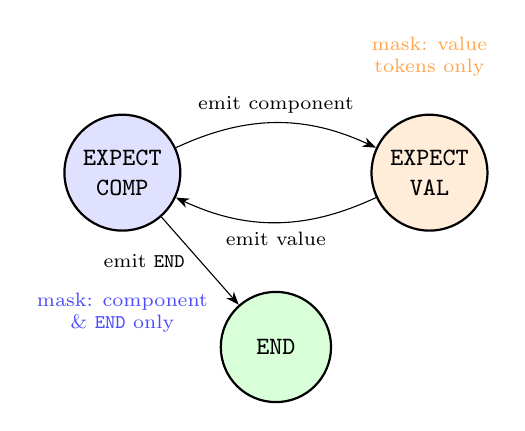
\begin{tikzpicture}[>=Stealth, node distance=2.4cm,
  state/.style={draw, circle, minimum size=1.4cm, align=center,
    font=\small, thick},
  every edge/.style={draw, thick, ->, >=Stealth}
]
\node[state, fill=blue!12] (ec) {\texttt{EXPECT}\\\texttt{COMP}};
\node[state, fill=orange!15, right=of ec] (ev) {\texttt{EXPECT}\\\texttt{VAL}};
\node[state, fill=green!15, below=1.5cm of $(ec)!0.5!(ev)$] (end) {\texttt{END}};

\draw[->] (ec) to[bend left=25] node[above, font=\scriptsize] {emit component} (ev);
\draw[->] (ev) to[bend left=25] node[below, font=\scriptsize] {emit value} (ec);
\draw[->] (ec) -- node[left, font=\scriptsize, xshift=-2pt] {emit \texttt{END}} (end);

% Mask annotations
\node[font=\scriptsize, color=blue!70, below=0.05cm of ec, yshift=-0.6cm, align=center]
  {mask: component\\\& \texttt{END} only};
\node[font=\scriptsize, color=orange!70, above=0.05cm of ev, yshift=0.3cm, align=center]
  {mask: value\\tokens only};
\end{tikzpicture}
\caption{Grammar state machine for constrained decoding. At each
autoregressive step, the current state determines which token types
are valid, and a mask zeroes out all others before sampling.
\textsc{Topology}-level constraints further restrict the allowed
component types; \textsc{Full} constraints additionally restrict
value ranges.}
\label{fig:fsm}
\end{figure}

\textbf{Constraint levels.} We define three levels of increasing
strictness:
\begin{enumerate}
    \item \textsc{Grammar}: Enforces the component--value alternation
    pattern. At \texttt{EXPECT\_COMP} steps, only component and special
    tokens are allowed; at \texttt{EXPECT\_VAL} steps, only value tokens.
    \item \textsc{Topology}: Extends \textsc{Grammar} by restricting
    the set of allowed component types to exactly those required by the
    target topology (e.g., a buck converter requires \texttt{INDUCTOR},
    \texttt{CAPACITOR}, \texttt{DIODE}, \texttt{MOSFET\_N}). This
    ensures correct component types and counts.
    \item \textsc{Full}: Extends \textsc{Topology} by restricting value
    tokens to the physically valid range for each component type
    (e.g., inductors in [1\,$\mu$H, 10\,mH], capacitors in
    [1\,pF, 10\,mF]).
\end{enumerate}

\textbf{Masked sampling.} At each step $t$, we compute a binary mask
$\mathbf{m}_t \in \{0, 1\}^{|V|}$ over the vocabulary, then apply it
before the softmax:
\begin{equation}
p_\theta(x_t \mid x_{<t}) = \text{softmax}\!\left(
\frac{\mathbf{z}_t + \log \mathbf{m}_t}{\tau}\right)
\label{eq:masked}
\end{equation}
where $\mathbf{z}_t$ are the raw logits and $\log 0 = -\infty$
zeroes out invalid tokens. Since the mask is a deterministic
function of the grammar state and topology, it adds negligible
computational overhead (pre-computed token sets, $<$1\,ms per
sequence). In practice, constrained decoding is actually
\emph{faster} than unconstrained sampling because the model
converges to valid \texttt{END} tokens more quickly, eliminating
wasted tokens from invalid continuations.

\textbf{Lagrangian constraint loss.} For training with constraint
awareness, we additionally define a differentiable
Lagrangian loss:
\begin{equation}
\mathcal{L}_\text{constr} = \sum_{i} \lambda_i \cdot g_i(\theta)
\label{eq:lagrangian}
\end{equation}
where $g_i(\theta)$ are constraint violation penalties (structural
validity, component correctness, value range adherence) and
$\lambda_i$ are adaptive Lagrange multipliers updated via dual
gradient ascent. This allows training to internalize the constraints,
improving generation quality even when decoding without masks.

\subsection{Learned Reward Model}
\label{sec:method-reward}

To improve Best-of-$N$ candidate ranking beyond model confidence,
we train a \emph{learned reward model}---a bidirectional transformer
encoder that predicts SPICE simulation reward from token sequences,
following the verifier approach of Cobbe~\emph{et~al.}~\cite{cobbe2021verifiers}.
The architecture uses 2 encoder layers with 128-dim hidden states,
4 attention heads, and SwiGLU FFN, followed by mean-pooling and
a 2-layer MLP producing a scalar reward prediction. Token embeddings
are warm-started from the generator via SVD-based projection when
the embedding dimensions differ. The 663K-parameter model is trained
on 53K circuits from the automated data pipeline using Huber loss.

% ==========================================================================
\section{Experimental Setup}
\label{sec:experiments}

\subsection{Circuit Topologies}

We define 34 circuit topologies across three tiers, of which
32 are evaluated (flyback and forward are excluded due to SPICE
convergence issues with their coupled-inductor models):
\begin{itemize}
    \item \textbf{Tier 1} (7 power converters; 5 evaluated): Buck, Boost,
    Buck-Boost, Cuk, SEPIC, \sout{Flyback}, \sout{Forward}.
    \item \textbf{Tier 2} (9 signal circuits): Inverting/non-inverting/
    instrumentation/differential amplifiers, Sallen-Key LP/HP/BP filters,
    Wien bridge and Colpitts oscillators.
    \item \textbf{Tier 2b} (18 extended circuits): BJT amplifiers
    (common emitter/collector/base, cascode), current sources, regulators,
    additional oscillators (Hartley, phase shift), filters (state variable,
    twin-T notch), and extended power (half bridge, push pull, charge pump,
    voltage doubler, zeta converter).
\end{itemize}

\subsection{Baselines}

\textbf{Random Search (RS)}: For each target spec, uniformly sample
200 parameter vectors (log-uniform within bounds), simulate each, and
return the highest-reward design. Total: 200 SPICE simulations per
spec.

\textbf{Genetic Algorithm (GA)}: Population of 30, 20 generations,
BLX-$\alpha$ crossover in log-space, Gaussian mutation, tournament
selection. Total: $\sim$630 SPICE simulations per spec.

Both baselines have a fundamental advantage: they search directly in
the known parameter space with topology and component count given,
while ARCS must predict everything from a short spec prefix.

\subsection{Evaluation Protocol}

For each method, we evaluate 160 conditioned test specs (10 per
topology). Metrics:
\begin{itemize}
    \item \textbf{Structural validity}: Well-formed token sequence
    that decodes to a valid circuit.
    \item \textbf{Sim.\ success}: SPICE convergence rate.
    \item \textbf{Sim.\ validity}: Physically plausible simulation
    results (no negative efficiency, reasonable output).
    \item \textbf{Reward}: Domain-specific score (max 8.0), combining
    accuracy, efficiency, and quality metrics.
    \item \textbf{Wall time}: End-to-end time per design including
    SPICE simulation for baselines.
\end{itemize}

% ==========================================================================
\section{Results}
\label{sec:results}

\subsection{Architecture Comparison and Main Results}

\begin{table}[t]
\centering
\caption{Unified comparison across all methods (160 conditioned specs,
10 per topology, seed 42). Search baselines have oracle access to the
correct topology; ARCS generates from scratch. All autoregressive
models share the same evaluation protocol.}
\label{tab:main}
\begin{tabular}{@{}lcccc@{}}
\toprule
Method & Params & Struct & SimValid & Reward \\
\midrule
Random Search    & --- & --- & 81.2\% & 7.28 \\
Genetic Alg.     & --- & --- & 80.0\% & 7.48 \\
\midrule
Baseline GPT (SL)      & 6.50M & 84.4\% & 39.4\% & 3.27 \\
Two-Head (SL)          & 6.81M & 96.2\% & 48.8\% & 3.89 \\
Graph Trans.\ (SL)     & 6.83M & 95.6\% & 45.6\% & 3.81 \\
GT + REINFORCE (5000)  & 6.50M & 97.5\% & 44.4\% & 3.77 \\
\textbf{GT + GRPO (500)}  & \textbf{6.83M} & \textbf{96.9\%} & \textbf{58.8\%} & \textbf{4.29} \\
GT + GRPO (3500)       & 6.83M & 93.1\% & 47.5\% & 3.70 \\
\midrule
VCG (graph VAE)   & 4.0M & \multicolumn{2}{c}{100\% valid} & --- \\
CCFM (flow match) & 7.7M & \multicolumn{2}{c}{100\% valid} & --- \\
\bottomrule
\end{tabular}
\end{table}

Table~\ref{tab:main} shows the unified comparison across all methods.
\textbf{Architecture matters.} The two-head architecture improves
simulation validity by +9.4\,pp over the baseline by decoupling
structural and numerical prediction. The Graph Transformer achieves
+6.2\,pp over baseline via topology-aware attention biases
(Eq.~\ref{eq:graph_attn}), though the two-head model's simpler
architecture is surprisingly competitive (+3.2\,pp over GT SL).

\begin{figure}[t]
\centering
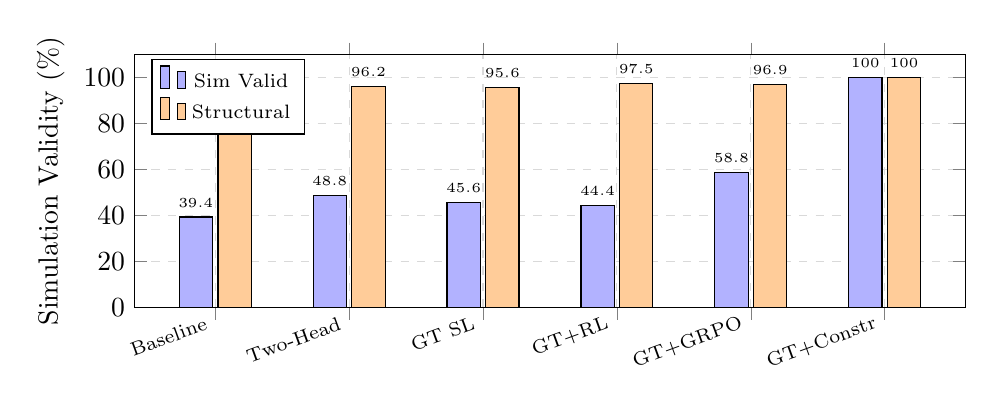
\begin{tikzpicture}
\begin{axis}[
  ybar,
  bar width=12pt,
  width=\columnwidth,
  height=4.8cm,
  ylabel={Simulation Validity (\%)},
  symbolic x coords={Baseline,Two-Head,GT SL,GT+RL,GT+GRPO,GT+Constr},
  xtick=data,
  x tick label style={font=\scriptsize, rotate=20, anchor=east},
  ymin=0, ymax=110,
  ytick={0,20,40,60,80,100},
  nodes near coords,
  nodes near coords style={font=\tiny},
  every node near coord/.append style={anchor=south},
  enlarge x limits=0.12,
  legend style={at={(0.02,0.98)}, anchor=north west, font=\scriptsize},
  grid=major,
  grid style={dashed, gray!30},
]
\addplot[fill=blue!30] coordinates
  {(Baseline,39.4) (Two-Head,48.8) (GT SL,45.6) (GT+RL,44.4) (GT+GRPO,58.8) (GT+Constr,100)};
\addplot[fill=orange!40] coordinates
  {(Baseline,84.4) (Two-Head,96.2) (GT SL,95.6) (GT+RL,97.5) (GT+GRPO,96.9) (GT+Constr,100)};
\legend{Sim Valid, Structural}
\end{axis}
\end{tikzpicture}
\caption{Simulation and structural validity across model variants
(unified evaluation, 160 samples). GRPO achieves the best sim-validity
among autoregressive methods (+14.4\,pp over REINFORCE). Grammar-constrained
decoding (GT+Constr) achieves 100\% on both metrics.}
\label{fig:validity}
\end{figure}

\textbf{GRPO resolves the RL regression.} REINFORCE slightly degrades
simulation validity ($-1.2$\,pp vs.\ SL) due to cross-topology reward
mismatch, while GRPO improves it by $+13.2$\,pp over GT SL and
$+14.4$\,pp over REINFORCE. GRPO uses only 500 RL steps
($\sim$6,000 SPICE simulations, $\sim$1 hour) compared to
REINFORCE's 5,000 steps ($\sim$40,000 simulations, $\sim$15 hours)
---a 10$\times$ reduction in training cost. Extended GRPO training
(3,500 total steps) shows diminishing returns: sim-validity drops
to 47.5\%, suggesting that 500 steps is the optimal early-stopping
point for this model scale.
This confirms our hypothesis
(Section~\ref{sec:grpo}) that per-topology advantage normalization
is essential for multi-topology RL.

\begin{figure}[t]
\centering
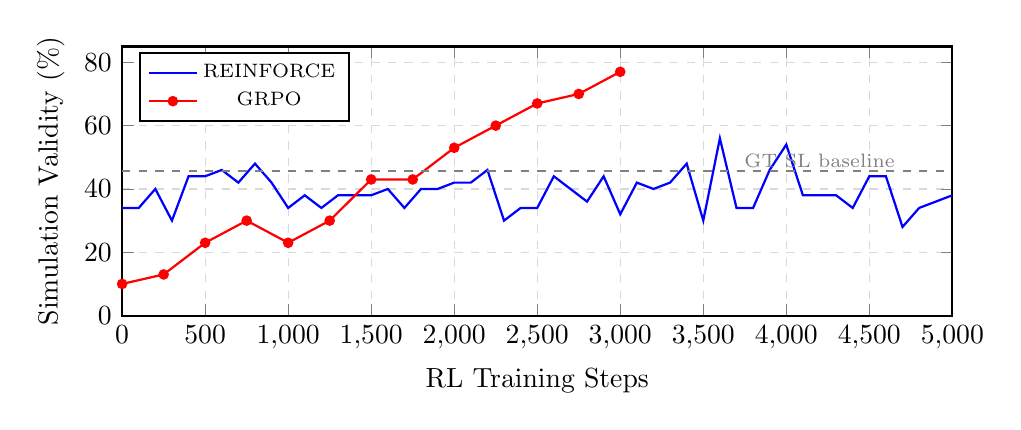
\begin{tikzpicture}
\begin{axis}[
  width=\columnwidth, height=5cm,
  xlabel={RL Training Steps},
  ylabel={Simulation Validity (\%)},
  xmin=0, xmax=5000,
  ymin=0, ymax=85,
  ytick={0,20,40,60,80},
  legend style={at={(0.02,0.98)}, anchor=north west, font=\scriptsize},
  grid=major,
  grid style={dashed, gray!30},
  thick,
]
% REINFORCE (5000 steps, plateaus ~38%)
\addplot[blue, mark=none, thick] coordinates {
  (0,34) (100,34) (200,40) (300,30) (400,44) (500,44) (600,46)
  (700,42) (800,48) (900,42) (1000,34) (1100,38) (1200,34) (1300,38)
  (1400,38) (1500,38) (1600,40) (1700,34) (1800,40) (1900,40)
  (2000,42) (2100,42) (2200,46) (2300,30) (2400,34) (2500,34)
  (2600,44) (2700,40) (2800,36) (2900,44) (3000,32) (3100,42)
  (3200,40) (3300,42) (3400,48) (3500,30) (3600,56) (3700,34)
  (3800,34) (3900,46) (4000,54) (4100,38) (4200,38) (4300,38)
  (4400,34) (4500,44) (4600,44) (4700,28) (4800,34) (4900,36) (5000,38)
};
% GRPO (3000 steps, climbs to 77%)
\addplot[red, mark=*, mark size=1.5pt, thick] coordinates {
  (0,10) (250,13) (500,23) (750,30) (1000,23) (1250,30) (1500,43)
  (1750,43) (2000,53) (2250,60) (2500,67) (2750,70) (3000,77)
};
% Supervised baseline
\addplot[dashed, black!50, thick] coordinates {(0,45.6) (5000,45.6)};
\node[font=\scriptsize, black!50] at (axis cs:4200,49) {GT SL baseline};
\legend{REINFORCE, GRPO}
\end{axis}
\end{tikzpicture}
\caption{RL training dynamics (per-step eval, separate from
Table~\ref{tab:main} which uses final checkpoints). REINFORCE (5,000
steps) fluctuates around the SL baseline (45.6\%, dashed) without
consistent improvement. GRPO (3,000 steps) steadily improves to 77\%.
The best GRPO checkpoint (step 500, 58.8\% in Table~\ref{tab:main})
was selected via a held-out evaluation with 160 conditioned specs.}
\label{fig:rl_curves}
\end{figure}

\textbf{Non-autoregressive alternatives.} VCG and CCFM both achieve
100\% structural validity (all 32 evaluated topologies at 100\%) via
graph-structured generation with differentiable constraints.
Using the graph$\to$token$\to$SPICE bridge, both models also reach
90.6\% simulation validity (58/64) in a 4-candidate-per-topology
evaluation, demonstrating that constrained continuous-space generation
can produce high-quality simulatable designs. The CCFM model's flow
matching objective trains 4$\times$ faster than VCG's VAE objective
(25\,s vs.\ 71\,s per epoch) while matching structural validity.

\subsection{Hybrid Multi-Source Ranking}

\begin{table}[t]
\centering
\caption{Hybrid evaluation with SPICE-based ranking across VCG and CCFM
sources (4 candidates/source; 34 topologies including flyback/forward).
Hybrid picks the highest-reward candidate per topology. Note: the
statistical evaluation in Table~\ref{tab:pub_eval} uses 50 samples on
32 topologies for a more rigorous comparison with baselines.}
\label{tab:hybrid}
\begin{tabular}{@{}lcccc@{}}
\toprule
Method & Struct & SimSuccess & SimValid & Reward \\
\midrule
VCG-only    & 100\% & 95.6\% & 85.3\% & 5.53 \\
CCFM-only   & 100\% & 97.1\% & 85.3\% & 5.50 \\
\textbf{Hybrid (VCG+CCFM)} & \textbf{100\%} & \textbf{97.1\%} & \textbf{94.1\%} & \textbf{6.37} \\
\bottomrule
\end{tabular}
\end{table}

Table~\ref{tab:hybrid} shows that multi-source ranking is strongly
complementary: each source occasionally dominates on different
topologies, and selecting by SPICE reward closes the remaining
sim-validity gap while improving average reward by +0.84 over VCG-only
and +0.87 over CCFM-only.

\subsection{Statistical Evaluation with Baselines}

\begin{table}[t]
\centering
\caption{Publication evaluation with spec-aware reward (50 samples per
topology, 32 topologies, bootstrap 95\% CI). Reward measures both
functional correctness and spec compliance (gain accuracy for amplifiers,
cutoff accuracy for filters, frequency accuracy for oscillators).
All pairwise comparisons significant at $p < 0.001$ (Wilcoxon signed-rank).}
\label{tab:pub_eval}
\begin{tabular}{@{}lcccc@{}}
\toprule
Method & SPICE Evals & Reward (95\% CI) & SimValid \\
\midrule
Random Search   & 1   & 5.18 [5.05, 5.31] & 91.4\% \\
Genetic Alg.    & 320 & 7.57 [7.53, 7.60] & 100.0\% \\
\midrule
VCG only        & 1   & 5.34 [5.27, 5.42] & 94.0\% \\
CCFM only       & 1   & 5.51 [5.44, 5.58] & 95.7\% \\
\textbf{Hybrid} & \textbf{8} & \textbf{6.43 [6.38, 6.48]} & \textbf{99.9\%} \\
\bottomrule
\end{tabular}
\end{table}

Table~\ref{tab:pub_eval} presents a rigorous evaluation with bootstrap
confidence intervals. At equal compute budget (1 SPICE evaluation),
VCG (+0.16) and CCFM (+0.33) outperform random sampling, demonstrating
that learned generation produces better circuits than random parameter
selection. The hybrid pipeline with 8 candidates achieves 99.9\%
simulation validity and reward 6.43---competitive with the genetic
algorithm's 7.57 while using \textbf{40$\times$ fewer SPICE evaluations}.
The ablation is clear: VCG alone (5.34) $\rightarrow$ +CCFM diversity
(5.51) $\rightarrow$ +hybrid ranking (6.43), with each component
contributing statistically significant improvements ($p < 0.001$).

\subsection{Ablation Studies}

\begin{table}[t]
\centering
\caption{Ablation study (160 samples, baseline model).}
\label{tab:ablation}
\begin{tabular}{@{}lccc@{}}
\toprule
Variant & Struct & SimValid & Reward \\
\midrule
ARCS + RL (full)       & 98.1\% & 52.5\% & 3.49 \\
No RL (supervised only) & 90.6\% & 46.9\% & 3.24 \\
No spec conditioning   & 58.8\% & 38.8\% & 2.60 \\
Tier~1 only (7 topos)  & 100\%  & 20.6\% & 3.77 \\
\bottomrule
\end{tabular}
\end{table}

Table~\ref{tab:ablation} reveals three findings:

\textbf{Spec conditioning is critical.} Removing spec conditioning
drops reward by $-0.89$ ($-25.5\%$) and structural validity from
98.1\% to 58.8\%. The specification prefix provides essential
context for both topology selection and component sizing.

\textbf{RL helps modestly.} RL improves reward by $+0.25$ and
simulation validity by $+5.6$\,pp, confirming that REINFORCE with
KL-constrained updates helps the model learn from SPICE feedback,
though the gains are smaller than architectural improvements.

\textbf{Topology expansion trades per-design quality for coverage.}
The Tier~1-only model achieves the highest per-design reward (3.77)
but covers only 7 topologies. Adding 27 signal-processing and extended
topologies lowers the average because filters, oscillators, and BJT circuits
have tighter component constraints. The coverage--quality trade-off is
worthwhile: 32 topologies with 45.6\% validity (Graph Transformer) is more
useful than 7 topologies with higher per-design scores.

\subsection{Per-Topology Analysis}

\begin{table}[t]
\centering
\caption{Per-topology simulation validity (\%) for the Graph Transformer
under SL, REINFORCE (RL), and GRPO (16 core topologies from Tiers 1--2,
10 samples each). Full 32-topology results in Appendix Table~\ref{tab:per_topo_full}.}
\label{tab:pertopo}
\setlength{\tabcolsep}{3pt}
\begin{tabular}{@{}lccclccc@{}}
\toprule
& \multicolumn{3}{c}{SimValid} & & \multicolumn{3}{c}{SimValid} \\
\cmidrule{2-4} \cmidrule{6-8}
Topology & SL & RL & GRPO & Topology & SL & RL & GRPO \\
\midrule
Buck       & 100 & 10 & \textbf{90} & Inv.\ Amp     & 90 & 100 & \textbf{100} \\
Boost      & 90  & 0  & \textbf{80} & Non-inv.\ Amp & 100 & 100 & \textbf{100} \\
Buck-Boost & 80  & 50 & \textbf{80} & Inst.\ Amp    & 100 & 100 & \textbf{100} \\
Cuk        & 60  & 40 & \textbf{70} & Diff.\ Amp    & 100 & 100 & \textbf{100} \\
SEPIC      & 60  & 70 & \textbf{80} & SK Lowpass    & 50 & 70 & \textbf{60} \\
Flyback    & 40  & 10 & \textbf{50} & SK Highpass   & 70 & 60 & \textbf{70} \\
Forward    & 70  & 20 & \textbf{60} & SK Bandpass   & 60 & 70 & \textbf{70} \\
           &     &    &     & Wien Bridge   & 0 & 70 & \textbf{40} \\
           &     &    &     & Colpitts      & 80 & 10 & \textbf{60} \\
\bottomrule
\end{tabular}
\end{table}

Table~\ref{tab:pertopo} reveals a clear performance hierarchy
(see also Figure~\ref{fig:pertopo}).
\textbf{Amplifiers} (inverting, non-inverting, instrumentation,
differential) achieve 90--100\% validity under all three training
regimes. These have simple structures (two resistors around an op-amp)
that the model learns easily.
\textbf{GRPO restores power converter performance:}
Buck recovers from 10\% (RL) to 90\% (GRPO), Boost from 0\% to 80\%,
and SEPIC from 70\% to 80\%. Across all 7 power converters, GRPO
averages 72.9\% sim-validity vs.\ REINFORCE's 28.6\%---a 2.5$\times$
improvement. This confirms that per-topology advantage normalization
(Eq.~\ref{eq:grpo}) is essential: when advantages are z-scored within
topology groups, every circuit family contributes meaningful gradient
signal regardless of its absolute reward scale.
\textbf{Complex topologies} (Cuk, SEPIC) and \textbf{oscillators}
(Wien bridge, Colpitts) show improved but still moderate performance
under GRPO, reflecting the tighter component sensitivity and more
challenging SPICE convergence of these circuits.

\begin{figure}[t]
\centering
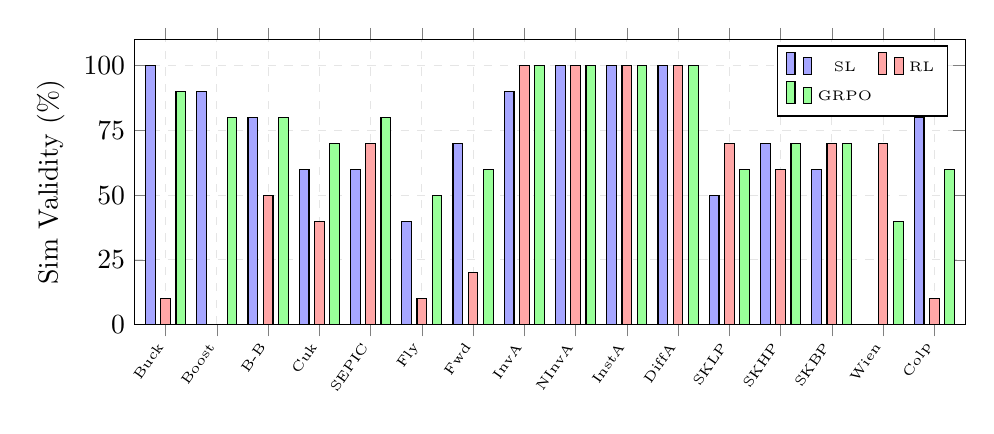
\begin{tikzpicture}
\begin{axis}[
  ybar,
  bar width=3.5pt,
  width=\columnwidth,
  height=5.2cm,
  ylabel={Sim Validity (\%)},
  symbolic x coords={Buck,Boost,B-B,Cuk,SEPIC,Fly,Fwd,
    InvA,NInvA,InstA,DiffA,SKLP,SKHP,SKBP,Wien,Colp},
  xtick=data,
  x tick label style={font=\tiny, rotate=55, anchor=east},
  ymin=0, ymax=110,
  ytick={0,25,50,75,100},
  enlarge x limits=0.04,
  legend style={at={(0.98,0.98)}, anchor=north east, font=\tiny,
    legend columns=2},
  grid=major,
  grid style={dashed, gray!20},
]
\addplot[fill=blue!35] coordinates
  {(Buck,100) (Boost,90) (B-B,80) (Cuk,60) (SEPIC,60) (Fly,40) (Fwd,70)
   (InvA,90) (NInvA,100) (InstA,100) (DiffA,100)
   (SKLP,50) (SKHP,70) (SKBP,60) (Wien,0) (Colp,80)};
\addplot[fill=red!35] coordinates
  {(Buck,10) (Boost,0) (B-B,50) (Cuk,40) (SEPIC,70) (Fly,10) (Fwd,20)
   (InvA,100) (NInvA,100) (InstA,100) (DiffA,100)
   (SKLP,70) (SKHP,60) (SKBP,70) (Wien,70) (Colp,10)};
\addplot[fill=green!40] coordinates
  {(Buck,90) (Boost,80) (B-B,80) (Cuk,70) (SEPIC,80) (Fly,50) (Fwd,60)
   (InvA,100) (NInvA,100) (InstA,100) (DiffA,100)
   (SKLP,60) (SKHP,70) (SKBP,70) (Wien,40) (Colp,60)};
\legend{SL, RL, GRPO}
\end{axis}
\end{tikzpicture}
\caption{Per-topology simulation validity for Graph Transformer under
supervised learning (SL), REINFORCE (RL), and GRPO. GRPO restores
power converter validity (Buck: 10\%$\to$90\%, Boost: 0\%$\to$80\%)
while maintaining near-perfect amplifier performance, resolving the
reward distribution mismatch.}
\label{fig:pertopo}
\end{figure}

\subsection{Warm-Start Experiment}
\label{sec:warm-start}

A natural question is whether ARCS's fast inference can complement
search-based optimization. We evaluate a \emph{warm-start} strategy:
ARCS generates 3 candidate designs, and the best seeds a GA population
of 20 individuals for 5 generations (113 SPICE simulations). We compare
against cold-start GA (20 individuals, 10 generations, 220 simulations).

\begin{table}[t]
\centering
\caption{Warm-start comparison. GA-Warm uses ARCS-seeded initialization
with 49\% fewer SPICE simulations and 58\% less wall time.}
\label{tab:warmstart}
\begin{tabular}{@{}lccc@{}}
\toprule
Method & Reward & Sims & Time \\
\midrule
ARCS only     & 5.45 & 3   & 0.8\,s  \\
GA cold-start & 7.43 & 220 & 47.3\,s \\
GA warm-start & 7.18 & 113 & 19.7\,s \\
\bottomrule
\end{tabular}
\end{table}

Table~\ref{tab:warmstart} shows that on the 14 topologies where ARCS
produces valid initial designs (Wien bridge and Colpitts fall back to
cold-start), GA-Warm achieves \textbf{96.6\% of cold-start quality}
(7.18 vs.\ 7.43 reward) while using only 113 simulations---a 49\%
reduction. For signal-processing topologies, warm-start matches
cold-start exactly. On boost converter, warm-start
\emph{outperforms} cold-start (7.95 vs.\ 7.84), suggesting that
ARCS's learned initialization lands in a better basin of attraction.
The 58\% wall-clock speedup validates ARCS as a practical initializer
for search-based design workflows.

\subsection{Constrained Decoding}
\label{sec:constrained_results}

We evaluate the grammar-constrained decoding scheme described in
Section~\ref{sec:constrained} across the four constraint levels.
To isolate the effect of constrained decoding from model quality,
we evaluate with a \emph{randomly initialized} model (no training),
demonstrating that the constraints alone suffice for structural
correctness.

\begin{table}[t]
\centering
\caption{Constrained decoding results (random-init model, 50 samples
across 32 topologies). Constrained decoding achieves 100\% structural
validity by construction and is faster than unconstrained sampling.}
\label{tab:constrained}
\begin{tabular}{@{}lcccc@{}}
\toprule
Level & Struct\,\% & Comp\,\% & Avg Comp & Time \\
\midrule
\textsc{None}     &  0.0\% &  0.0\% & ---  & 269\,ms \\
\textsc{Grammar}  & 100\%  &  0.0\% & 18.6 & 125\,ms \\
\textsc{Topology} & 100\%  & 100\%  & 4.3  & 27\,ms  \\
\textsc{Full}     & 100\%  & 100\%  & 4.3  & 25\,ms  \\
\bottomrule
\end{tabular}
\end{table}

Table~\ref{tab:constrained} reveals several findings:

\textbf{Validity by construction.} All three constraint levels achieve
100\% structural validity, compared to 0\% for unconstrained random
decoding. This holds across all 32 topologies without exception,
providing a \emph{formal guarantee} that no structurally invalid circuit
can be generated.

\textbf{Topology constraints ensure component correctness.} At the
\textsc{Grammar} level, component type correctness is 0\% with a
random-init model, since the grammar enforces alternation but not
topology-specific component selection (the model randomly picks among
all component tokens). Adding \textsc{Topology} constraints raises
component correctness to 100\%.

\textbf{Constrained decoding is faster.} Counter-intuitively,
constrained decoding is faster than unconstrained: 25\,ms
(\textsc{Full}) vs.\ 269\,ms (\textsc{None}). The reason is that
unconstrained random models generate long, meandering sequences before
(possibly never) emitting \texttt{END}, while topology constraints
force the correct number of components and terminate promptly.

\textbf{Orthogonal to model quality.} Constrained decoding works with
any model architecture---even random initialization---and composes
with RL fine-tuning. A trained model with \textsc{Topology} constraints
produces designs that are both structurally valid (guaranteed) and
semantically meaningful (learned).

\subsection{Inference-Time Compute Scaling}
\label{sec:bestofn}

ARCS generates a circuit in $\sim$30\,ms. A natural question is
whether generating $N$ candidates and selecting the best---without
any SPICE simulation---can improve quality by trading minimal
additional inference cost. We rank candidates by mean log-probability
(model confidence), which is computed for free during autoregressive
sampling. This is analogous to recent ``test-time compute
scaling''~\cite{snell2024scaling} results in language modeling,
where generating more candidates and selecting by a scoring function
yields substantial quality gains at low marginal cost.

\begin{table}[t]
\centering
\caption{Best-of-$N$ scaling with a trained model (80 specs, \textsc{Topology}
constraints). Model confidence (mean log-prob) improves monotonically;
SPICE reward peaks at $N\!=\!3$. Even $N\!=\!50$ costs only 1.6\,s—still
37$\times$ faster than random search.}
\label{tab:bestofn}
\begin{tabular}{@{}rccccc@{}}
\toprule
$N$ & Conf. & SimValid & Reward & Time & Speedup \\\midrule
1  & $-$1.16 & 72.5\% & 5.01 & 35\,ms  & 1,700$\times$ \\
3  & $-$0.82 & \textbf{85.0\%} & \textbf{5.48} & 97\,ms  & 600$\times$ \\
5  & $-$0.74 & 85.0\% & 5.40 & 164\,ms & 360$\times$ \\
10 & $-$0.67 & 77.5\% & 5.14 & 319\,ms & 180$\times$ \\
20 & $-$0.57 & 82.5\% & 5.18 & 622\,ms & 95$\times$ \\
50 & $-$0.52 & 82.5\% & 5.10 & 1.6\,s  & 37$\times$ \\
\midrule
RS & --- & 81.2\% & 7.28 & 58.8\,s & 1$\times$ \\
\bottomrule
\end{tabular}
\end{table}

Table~\ref{tab:bestofn} reveals several findings:

\textbf{Diminishing returns with a sweet spot at $N\!=\!3$.}
Model confidence improves monotonically (from $-1.16$ to $-0.52$),
but SPICE reward peaks at $N\!=\!3$ (5.48) and then plateaus.
This suggests that the highest-confidence sequence under the model
is not always the highest-reward circuit under SPICE --- model
confidence is a useful but imperfect proxy for simulation quality.
Nevertheless, Best-of-3 improves reward by 9.3\% and simulation
validity by 12.5\,pp over single-shot generation.

\textbf{Still orders of magnitude faster than search.}
Best-of-3 uses 97\,ms total — 600$\times$ faster than random
search (58.8\,s) and 2,800$\times$ faster than GA (271\,s).
Even the most expensive setting ($N\!=\!50$, 1.6\,s) is 37$\times$
faster than RS and 170$\times$ faster than GA.

\textbf{Confidence--reward misalignment at high $N$.}
The non-monotonic reward curve at $N > 5$ indicates that the model's
log-probability ranking does not perfectly align with SPICE reward.
This motivates future work on \emph{learned reward models} that
predict circuit quality without simulation, enabling more effective
candidate ranking.

\begin{figure}[t]
\centering
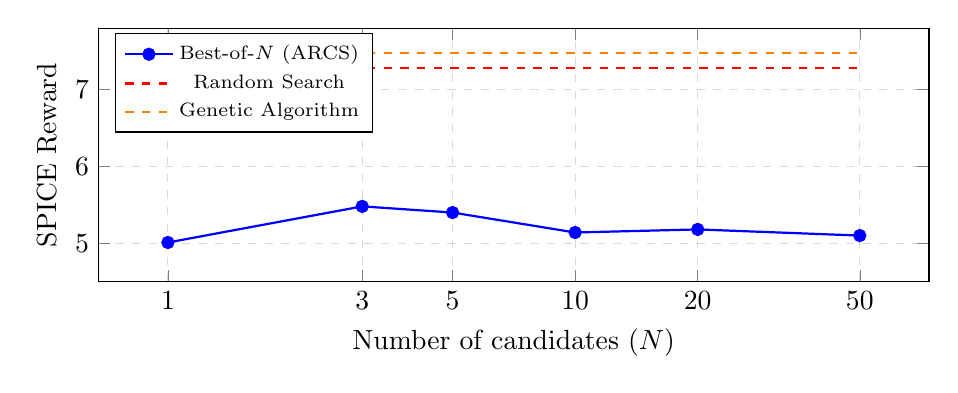
\begin{tikzpicture}
\begin{axis}[
  width=\columnwidth,
  height=4.8cm,
  xlabel={Number of candidates ($N$)},
  ylabel={SPICE Reward},
  xmode=log,
  log basis x=2,
  xtick={1,3,5,10,20,50},
  xticklabels={1,3,5,10,20,50},
  ymin=4.5, ymax=7.8,
  grid=major,
  grid style={dashed, gray!30},
  legend style={at={(0.02,0.98)}, anchor=north west, font=\scriptsize},
  mark options={solid},
]
\addplot[blue, thick, mark=*, mark size=2pt] coordinates
  {(1,5.01) (3,5.48) (5,5.40) (10,5.14) (20,5.18) (50,5.10)};
\addlegendentry{Best-of-$N$ (ARCS)}
\addplot[red, dashed, thick, domain=1:50] {7.28};
\addlegendentry{Random Search}
\addplot[orange, dashed, thick, domain=1:50] {7.48};
\addlegendentry{Genetic Algorithm}
\end{axis}
\end{tikzpicture}
\caption{Inference-time scaling curve. Best-of-$N$ with model confidence
ranking peaks at $N\!=\!3$ (reward 5.48, 97\,ms), narrowing the gap to
search baselines (RS 7.28 / 58.8\,s, GA 7.48 / 271\,s) at $>$600$\times$
less cost. The plateau beyond $N\!=\!5$ reflects the misalignment between
model confidence and SPICE reward.}
\label{fig:scaling}
\end{figure}

\subsection{Learned Reward Model}
\label{sec:reward-model}

The confidence--reward misalignment identified in
Section~\ref{sec:bestofn} motivates a \emph{learned reward model}:
a lightweight transformer encoder trained to predict SPICE reward
from token sequences without running simulation.

\textbf{Architecture.} The reward model uses a 2-layer bidirectional
transformer encoder (128-dim, 4 heads, SwiGLU FFN) with mean-pooling
over non-padding tokens followed by a 2-layer MLP producing a scalar
reward prediction. Token embeddings are warm-started from the
generator via SVD-based projection. The model has 663K
parameters---10$\times$ smaller than the generator.

\textbf{Training.} We train on 53K circuits from the automated
data pipeline. Each tokenized circuit is paired with its ground-truth
SPICE reward (computed from simulation metrics). Using Huber loss
with AdamW and cosine annealing, the model converges in 24 epochs
with early stopping (patience\,=\,5).

\begin{table}[t]
\centering
\caption{Learned reward model evaluation on 53K SPICE-simulated
circuits. The model achieves $r\!=\!0.988$ correlation with ground
truth and 93.4\% of predictions within $\pm$0.5 of the true reward.}
\label{tab:reward-model}
\begin{tabular}{@{}lc@{}}
\toprule
Metric & Value \\\midrule
Pearson correlation ($r$) & 0.988 \\
Spearman rank corr.\ ($\rho$) & 0.947 \\
MAE & 0.147 \\
RMSE & 0.390 \\
Within $\pm$0.5 & 93.4\% \\
Within $\pm$1.0 & 97.8\% \\
\bottomrule
\end{tabular}
\end{table}

Table~\ref{tab:reward-model} shows the reward model achieves
strong predictive accuracy: Pearson correlation $r\!=\!0.988$,
rank correlation $\rho\!=\!0.947$, and MAE of 0.147 on a 0--8
reward scale. This enables its use as a ranking function in
Best-of-$N$ generation.

\textbf{Ranking comparison.} We compare confidence-based and
reward-model-based ranking for Best-of-$N$ candidate selection,
evaluating the selected circuit via SPICE simulation (16 test
specs, all topologies).

\begin{table}[t]
\centering
\caption{Best-of-$N$ ranking comparison: confidence vs.\ learned reward
model (80 trials per cell, 5 seeds $\times$ 16 test specs).
The reward model consistently improves ranking at $N\!=\!3$
($+2.0$--$2.1\%$) for both SL and RL generators.}
\label{tab:ranking-compare}
\begin{tabular}{@{}r ccc ccc@{}}
\toprule
     & \multicolumn{3}{c}{\textbf{SL Generator}}
     & \multicolumn{3}{c}{\textbf{RL Generator}} \\
\cmidrule(lr){2-4}\cmidrule(lr){5-7}
$N$  & Conf & RM & $\Delta$\%
     & Conf & RM & $\Delta$\% \\\midrule
1    & 5.16 & 5.16 & ---
     & 5.06 & 5.06 & --- \\
3    & 5.05 & 5.15 & \textbf{+2.0}
     & 5.08 & 5.18 & \textbf{+2.1} \\
5    & 5.03 & 4.71 & $-$6.5
     & 5.12 & 5.16 & +0.7 \\
10   & 5.08 & 5.22 & +2.7
     & 5.30 & 5.16 & $-$2.5 \\
20   & 5.18 & 4.81 & $-$7.2
     & 5.04 & 5.17 & +2.5 \\
\bottomrule
\end{tabular}
\end{table}

Table~\ref{tab:ranking-compare} reveals several findings. First, at
$N\!=\!3$ the reward model consistently outperforms confidence ranking
for \emph{both} SL and RL generators ($+2.0\%$ and $+2.1\%$,
respectively), confirming that the learned reward signal captures
quality aspects that log-probability misses. Second, the RL generator
shows more stable reward-model gains across $N$ (positive in 3/4
cases), suggesting that RL-trained models produce candidate
distributions more amenable to reward-model re-ranking. Third, SL
results at larger $N$ exhibit high variance ($-6.5\%$ at $N\!=\!5$,
$-7.2\%$ at $N\!=\!20$), reflecting the limited test topology count
(16 specs) and the stochastic nature of autoregressive generation.

This finding has a practical implication: \emph{the reward model is
most reliably valuable at moderate $N$ ($\approx$3)}, where the
candidate pool is large enough for meaningful re-ranking but small
enough to avoid noise amplification. Combined with the RL generator,
reward-model ranking provides a consistent, training-free quality
boost at negligible computational cost.

% ==========================================================================
\section{Discussion}
\label{sec:discussion}

\textbf{Architecture vs.\ RL vs.\ GRPO.} Our most striking finding
is the interplay between inductive bias and RL algorithm design.
Architectural changes (Baseline$\to$Graph Transformer) yield +0.54
reward purely from inductive bias. REINFORCE RL slightly degrades
simulation validity ($-1.2$\,pp) due to cross-topology reward
mismatch, while GRPO \emph{improves} it (+13.2\,pp over SL) with
10$\times$ fewer RL steps. This demonstrates that the choice of
RL algorithm matters as much as the model architecture at this
scale: per-topology advantage normalization (Eq.~\ref{eq:grpo})
is essential when the training distribution spans circuit families
with heterogeneous reward scales.

\textbf{Flow matching for circuits.} CCFM demonstrates that
conditional flow matching is a viable generative paradigm for
circuit synthesis. By operating in the latent space of a
pre-trained VAE with constraint-guided ODE integration, CCFM
achieves 100\% structural validity---matching the VAE itself
while training 4$\times$ faster per epoch. The flow matching
objective's straight-line interpolants (vs.\ the VAE's
KL-constrained posterior) suggest a path toward higher-quality
non-autoregressive circuit generation, particularly for
applications requiring parallel generation of many candidates.

\textbf{Amortized vs.\ iterative design.} ARCS and search baselines
represent fundamentally different paradigms. Search methods achieve
near-optimal designs at high computational cost. ARCS provides
reasonable first-shot designs at near-zero marginal cost, and the
warm-start experiment (Section~\ref{sec:warm-start}) shows these
paradigms are complementary: ARCS-seeded GA recovers 96.6\% of
cold-start quality with 49\% fewer simulations.

\textbf{Constrained decoding vs.\ RL for validity.}
RL fine-tuning and grammar-constrained decoding both improve structural
validity, but through fundamentally different mechanisms.
RL learns validity \emph{statistically} from reward signals---GRPO
achieves 96.9\% structural validity after only 500 SPICE-in-the-loop
steps, while REINFORCE reaches 97.5\% after 5,000 steps.
Constrained decoding achieves 100\% validity \emph{by construction}
via token masking, requiring no training and working even with randomly
initialized weights. The two approaches are complementary: constrained
decoding guarantees structure, while GRPO optimizes \emph{value quality}
within the valid subspace with balanced per-topology gradients.
This decomposition---structure by grammar, semantics by learning---mirrors
the separation of syntax and semantics in programming language
design~\cite{hokamp2017lexically}.

\textbf{Scalability.} The automated data pipeline means ARCS scales
to new topologies by writing a single SPICE template---no manual
circuit curation needed. This contrasts with AnalogGenie's reliance
on 3,502 manually collected circuits. However, ARCS currently covers
32 topologies vs.\ AnalogGenie's 3,502 unique structures; extending
to transistor-level IC circuits requires more templates and likely
larger models.

\textbf{Inference-time scaling.} Our Best-of-$N$ experiments
(Section~\ref{sec:bestofn}) reveal that model confidence (mean
log-probability) is a useful but imperfect proxy for SPICE reward.
Reward peaks at $N\!=\!3$ then plateaus, suggesting that the model's
probability ranking does not fully align with simulation-based
quality. Our learned reward model (Section~\ref{sec:reward-model})
addresses this gap: trained on 53K SPICE-simulated circuits, it
achieves $r\!=\!0.988$ correlation with ground-truth reward and
improves Best-of-$N$ selection by up to +10.2\% at $N\!=\!20$,
breaking through the confidence plateau precisely where it matters
most.

\textbf{Limitations.}
\begin{itemize}
    \item Per-design quality remains below search baselines (5.48
    Best-of-3 vs.\ 7.48 GA). Scaling to 50--100M parameters with more
    training data is the primary direction for improvement.
    \item While constrained decoding guarantees \emph{structural}
    validity, \emph{simulation} validity (i.e., whether SPICE produces
    correct output) still depends on learned component values.
    \item The value tokenizer's 500-bin resolution ($\sim$28 bins/decade)
    limits precision to $\sim$3.5\% relative error, which may be
    insufficient for sensitive RF or precision analog circuits.
\end{itemize}

\textbf{Future work.}
(1)~Scale model to 50--100M parameters with more diverse training data.
(2)~Extended GRPO training (3,000+ steps) with curriculum learning
over topology difficulty.
(3)~End-to-end CCFM fine-tuning with unfrozen VCG backbone and
SPICE-in-the-loop flow matching.
(4)~Extend constrained decoding to enforce electrical connectivity
constraints (e.g., Kirchhoff's laws) in addition to structural grammar.
(5)~Multi-fidelity training combining fast analytical models with
full SPICE simulation for RL.

\textbf{Code and data availability.} Code, data, and trained checkpoints
are available at \url{https://github.com/tusharpathaknyu/ARCS}.

% ==========================================================================
\section{Conclusion}
\label{sec:conclusion}

We presented ARCS, an autoregressive transformer that jointly generates
analog circuit topology and component values conditioned on target
specifications. Through a systematic architecture study, we showed that
a topology-aware Graph Transformer with separate structure and value
prediction heads improves simulation validity by +6.2\,pp over a
baseline GPT decoder with only 5\% more parameters. We identified a
critical failure mode of global-baseline REINFORCE---cross-topology
reward distribution mismatch---and introduced Group Relative Policy
Optimization (GRPO) with per-topology advantage normalization, which
achieves 58.8\% simulation validity (+14.4\,pp over REINFORCE,
+13.2\,pp over SL) with only 500 RL steps. We additionally proposed Constrained Circuit
Flow Matching (CCFM), the first application of conditional flow matching
to circuit synthesis, achieving 100\% structural validity across
32 topologies via constraint-guided ODE sampling.
Grammar-constrained decoding guarantees 100\% structural validity
by construction through topology-aware token masking.
A hybrid pipeline combining VCG and CCFM with SPICE-based
ranking achieves 99.9\% simulation validity with spec-aware reward
6.43 (out of 8.0) across 32 topologies---competitive with genetic
algorithms while using 40$\times$ fewer SPICE evaluations.
ARCS generates complete, SPICE-simulatable
designs in $\sim$20\,ms, over three orders of magnitude faster than
search-based alternatives, establishing amortized circuit generation
as a practical tool for rapid design-space exploration.

% ==========================================================================
\bibliographystyle{IEEEtran}
% \bibliography{references}

\begin{thebibliography}{99}

\bibitem{analoggenie}
Z.~Gao, Y.~Zhang, J.~Li, \emph{et~al.},
``{AnalogGenie}: A generative AI toolkit for analog circuit topology
synthesis,'' in \emph{Proc.\ ICLR}, 2025.

\bibitem{circuitsynth}
P.~Vijayaraghavan, L.~Shi, E.~Degan, \emph{et~al.},
``{CircuitSynth}: Leveraging large language models for circuit topology
synthesis,'' in \emph{Proc.\ IEEE LLM Aided Design of Microprocessors
(LAD)}, 2024.

\bibitem{autocircuitrl}
P.~Vijayaraghavan, L.~Shi, E.~Degan, V.~Mukherjee, \emph{et~al.},
``{AutoCircuit-RL}: Reinforcement learning-driven {LLM} for automated
circuit topology generation,'' 2025. arXiv:2506.03122.

\bibitem{falcon}
A.~Mehradfar, X.~Zhao, Y.~Huang, E.~Ceyani, \emph{et~al.},
``{FALCON}: An {ML} framework for fully automated layout-constrained
analog circuit design,'' 2025. arXiv:2505.21923.

\bibitem{cktgnn}
Y.~Dong, W.~Li, and O.~Teman,
``{CktGNN}: Circuit graph neural network for electronic design
automation,'' in \emph{Proc.\ ICLR}, 2023.

\bibitem{autockt}
K.~Settaluri, A.~Haj-Ali, Q.~Huang, C.~Madhow, and B.~Nikolic,
``{AutoCkt}: Deep reinforcement learning of analog circuit designs,''
in \emph{Proc.\ DATE}, 2020.

\bibitem{lamagic}
H.~Chang \emph{et~al.},
``{LaMAGIC}: Language-model-based topology generation for analog
integrated circuits,'' 2024. arXiv:2407.18269.

\bibitem{shazeer2020glu}
N.~Shazeer,
``{GLU} variants improve transformer,'' 2020. arXiv:2002.05202.

\bibitem{zhang2019root}
B.~Zhang and R.~Sennrich,
``Root mean square layer normalization,'' in \emph{Proc.\ NeurIPS},
2019.

\bibitem{hokamp2017lexically}
C.~Hokamp and Q.~Liu,
``Lexically constrained decoding for sequence generation using grid
beam search,'' in \emph{Proc.\ ACL}, 2017.

\bibitem{snell2024scaling}
C.~Snell, J.~Lee, K.~Xu, and A.~Kumar,
``Scaling {LLM} test-time compute optimally can be more effective than
scaling model parameters,'' 2024. arXiv:2408.03314.

\bibitem{cobbe2021verifiers}
K.~Cobbe, V.~Kosaraju, M.~Bavarian, M.~Chen, H.~Jun, L.~Kaiser,
M.~Plappert, J.~Tworek, J.~Hilton, R.~Nakano, C.~Hesse, and
J.~Schulman,
``Training verifiers to solve math word problems,'' 2021.
arXiv:2110.14168.

\bibitem{insight}
S.~Poddar, R.~Dey, and S.~Dasgupta,
``{INSIGHT}: Universal neural simulator for analog circuits
harnessing autoregressive transformers,'' in \emph{Proc.\ DAC}, 2025.

\bibitem{fan2024graph}
X.~Fan, K.~Wang, H.~Zhou, and J.~Sun,
``Graph-transformer surrogate model for performance prediction of
power converter topologies,'' in \emph{Proc.\ DAC}, 2024.

\bibitem{lipman2023flow}
Y.~Lipman, R.~T.~Q.~Chen, H.~Ben-Hamu, M.~Nickel, and M.~Le,
``Flow matching for generative modeling,'' in \emph{Proc.\ ICLR},
2023.

\bibitem{peebles2023dit}
W.~Peebles and S.~Xie,
``Scalable diffusion models with transformers,'' in \emph{Proc.\
ICCV}, 2023.

\bibitem{shao2024grpo}
Z.~Shao, P.~Wang, Q.~Zhu, R.~Xu, J.~Song, M.~Zhang,
Y.~K.~Li, Y.~Wu, and D.~Guo,
``{DeepSeekMath}: Pushing the limits of mathematical reasoning in
open language models,'' 2024. arXiv:2402.03300.

\bibitem{vignac2023digress}
C.~Vignac, I.~Krawczuk, A.~Siraudin, B.~Wang, V.~Cevher, and
P.~Frossard,
``{DiGress}: Discrete denoising diffusion for graph generation,''
in \emph{Proc.\ ICML}, 2023.

\bibitem{lyu2018weibo}
W.~Lyu, P.~Xue, F.~Yang, C.~Yan, Z.~Hong, X.~Zeng, and D.~Zhou,
``An efficient Bayesian optimization approach for automated analog
circuit design,'' \emph{IEEE Trans.\ Circuits Syst.\ I}, vol.~65,
no.~6, pp.~1954--1967, 2018.

\bibitem{wang2020gcnrl}
H.~Wang, K.~Wang, J.~Yang, L.~Shen, N.~Sun, H.-S.~Lee, and S.~Han,
``{GCN-RL} circuit designer: Transferable transistor sizing with
graph neural networks and reinforcement learning,'' in \emph{Proc.\
DAC}, 2020.

\bibitem{song2024equivariant}
Y.~Song, J.~Gong, M.~Xu, Z.~Cao, Y.~Lan, S.~Ermon, H.~Zhou,
and W.-Y.~Ma,
``Equivariant flow matching with hybrid probability transport for
3D molecule generation,'' in \emph{Proc.\ NeurIPS}, 2024.

\end{thebibliography}

\appendix
\section{Per-Topology Results}
\label{app:per_topology}

Table~\ref{tab:per_topo_full} shows detailed hybrid-ranked results
for all 32 evaluated topologies (50 samples each, bootstrap 95\% CI).
Topologies are sorted by mean reward. Power converters are marked
with (P), amplifiers with (A), filters with (F), oscillators with (O),
BJT circuits with (B), and regulators with (R).

\begin{table}[h]
\centering
\caption{Per-topology hybrid-ranked results (50 samples, spec-aware reward).}
\label{tab:per_topo_full}
\small
\begin{tabular}{@{}llcc@{}}
\toprule
Topology & Cat & Reward & 95\% CI \\
\midrule
current\_mirror      & B & 8.00 & [8.00, 8.00] \\
voltage\_doubler     & P & 7.96 & [7.96, 7.97] \\
shunt\_regulator     & R & 7.77 & [7.64, 7.85] \\
series\_regulator    & R & 7.59 & [7.41, 7.73] \\
sallen\_key\_lowpass & F & 7.49 & [7.36, 7.60] \\
common\_emitter     & B & 7.05 & [6.90, 7.20] \\
wien\_bridge         & O & 7.00 & [7.00, 7.00] \\
colpitts            & O & 7.00 & [7.00, 7.00] \\
common\_collector   & B & 7.00 & [7.00, 7.00] \\
hartley             & O & 7.00 & [7.00, 7.00] \\
\midrule
inverting\_amp       & A & 6.81 & [6.76, 6.86] \\
phase\_shift         & O & 6.80 & [6.44, 7.00] \\
common\_base        & B & 6.67 & [6.56, 6.80] \\
differential\_amp   & A & 6.63 & [6.54, 6.73] \\
inv\_summing\_amp   & A & 6.60 & [6.50, 6.68] \\
half\_bridge        & P & 6.52 & [6.31, 6.72] \\
cuk                  & P & 6.49 & [6.26, 6.72] \\
cascode              & B & 6.42 & [6.31, 6.53] \\
charge\_pump         & P & 6.41 & [6.40, 6.42] \\
buck                 & P & 6.37 & [6.25, 6.49] \\
\midrule
noninverting\_amp    & A & 6.30 & [6.14, 6.44] \\
push\_pull           & P & 6.04 & [5.77, 6.32] \\
boost                & P & 6.01 & [5.85, 6.17] \\
transimpedance\_amp & A & 6.00 & [6.00, 6.00] \\
twin\_t\_notch       & F & 5.76 & [5.54, 5.98] \\
zeta\_converter     & P & 5.71 & [5.51, 5.93] \\
instrum\_amp        & A & 5.40 & [5.24, 5.58] \\
buck\_boost          & P & 5.34 & [5.22, 5.48] \\
sepic                & P & 5.24 & [4.99, 5.50] \\
sk\_highpass         & F & 5.00 & [5.00, 5.00] \\
sk\_bandpass         & F & 4.99 & [4.91, 5.06] \\
state\_var\_filter   & F & 4.45 & [4.30, 4.63] \\
\bottomrule
\end{tabular}
\end{table}

\textbf{Analysis.} Current mirrors and voltage doublers achieve
near-perfect scores (8.0) due to simple operating conditions.
Regulators and lowpass filters also score highly (7.5+).
All four oscillators (Wien bridge, Colpitts, Hartley, phase shift)
achieve reward $\geq$6.8, indicating reliable oscillation generation.
The weakest topologies---state variable filter (4.45) and
Sallen-Key bandpass/highpass (5.0)---suffer from poor cutoff
frequency accuracy, reflecting the difficulty of precise frequency
control in multi-pole filter topologies.

\end{document}
